\documentclass[twocolumn,landscape,10pt]{article}
\usepackage[thinc]{esdiff} % for typesettign derivatives
\usepackage{amsthm} % provides an enhanced version of LaTex's \newtheorem command
\usepackage{mdframed} % framed environments that can split at page boundaries
\usepackage{enumitem} % bulletin points or other means of listing things
\usepackage{amssymb} % for AMS symbols
\usepackage{amsmath} % so as to use align
\usepackage{latexsym} % so as to use symbols like \leadsto
\usepackage{mathrsfs} % for using mathscr for char like operators
\usepackage{commath} % for using norm symbol
\usepackage{mathtools} % for using environments like dcases
\usepackage{authblk} % for writing affiliations
\usepackage{graphicx} % for importing images
\graphicspath{{./images/}} % for the path to images, also always put label behind captions
\usepackage{textcomp} % for using degree symbol
\usepackage{hyperref} % for clickable link in the pdf & customizable reference text
\usepackage[all]{hypcap} % for clickable link to images instead of caption
\usepackage[margin=1.0in]{geometry} % default is 1.5in
% \usepackage[left=0.4in, right=0.4in, top=0.8in, bottom=0.8in]{geometry}
\usepackage[title]{appendix} % for attaching appendix
\allowdisplaybreaks % allow page breaking in display maths, like align
\usepackage{xcolor} % for setting color of a block of text, use \textcolor{<color>}{}
\usepackage[normalem]{ulem} % for strikethrough text, use \sout{}
% allow for more advanced table layout
\usepackage{booktabs}
\usepackage{multirow}
\usepackage{siunitx}
% for adjusting caption settings
\usepackage[justification=centering]{caption}
\captionsetup[table]{skip=10pt}

\theoremstyle{definition}
\mdfdefinestyle{defEnv}{%
  hidealllines=false,
  nobreak=true,
  innertopmargin=-1ex,
}

% The following is for writing block of code
\usepackage{listings}
\usepackage{color}

\definecolor{dkgreen}{rgb}{0,0.6,0}
\definecolor{gray}{rgb}{0.5,0.5,0.5}
\definecolor{mauve}{rgb}{0.58,0,0.82}

% setting of the thickness of the 4 lines of box
\setlength{\fboxrule}{2pt}

% Use the following to change code language and related settings
\lstset{frame=tb,
  language=Python,
  aboveskip=3mm,
  belowskip=3mm,
  showstringspaces=false,
  columns=flexible,
  basicstyle={\small\ttfamily},
  numbers=none,
  numberstyle=\tiny\color{gray},
  keywordstyle=\color{blue},
  commentstyle=\color{dkgreen},
  stringstyle=\color{mauve},
  breaklines=true,
  breakatwhitespace=true,
  tabsize=3,
  literate={~} {$\sim$}{1}
}

\pagestyle{headings}
\author{Lectured by Bernhard Kainz and Abhijeet Ghosh}
\title{Graphics}
\affil{Typed by Aris Zhu Yi Qing}
\begin{document}
\maketitle
\tableofcontents

\newpage
\section{Projections and Transformations}

\subsection{Parallel Projection}

\begin{itemize}
    \item For a vertex $\mathbf{V} = (V_x,V_y, V_z)^T$, the
        \underline{\textbf{projector}}
        (projection line) is defined by the parametric line equation
        \[
            \mathbf{P}=\mathbf{V}+\mu \mathbf{d}
        \]
    \item Assuming the projection plane is $z=0$, we can establish
        \[
            0 = P_z = V_z + \mu d_z
        \]
        to obtain $\mu$, thereby computing $P_x$ and $P_y$.
    \item \underline{\textbf{Orthographic projection}} is a special type of
        parallel projection:
        \begin{itemize}
            \item projection plane: $z=0$
            \item $\mathbf{d}=\begin{pmatrix}
                    0 & 0 & -1
                \end{pmatrix}^T$
            \item  $P_x=V_x$, $P_y=V_y$
        \end{itemize} 
\end{itemize} 

\subsection{Perspective Projections}

\begin{itemize}
    \item The \underline{\textbf{centre of projection}} is the viewpoint, which
        all the projectors pass through, assumed to be at the origin.
    \item For a vertex $\mathbf{V} = (V_x,V_y, V_z)^T$, the projector
        $\mathbf{P}$ has the equation
        \[
            \mathbf{P}=\mu\mathbf{V}
        \]
    \item Since the projection plane is at a constant $z$ value $f$, at the
        point of intersection we have
        \[
            f = P_z = \mu V_z
        \]
        to obtain $\mu$, thereby computing $P_x$ and $P_y$.
\end{itemize} 

\subsection{Space Transformations}

\subsubsection{Homogeneous Coordinates}

\begin{itemize}
    \item A \underline{\textbf{homogeneous coordinate}} is a three-dimensional
        coordinate with a fourth componenet called
        \underline{\textbf{ordinate}} which acts as a scale factor.
    \item Assuming a point $\mathbf{P}=(p_x,p_y,p_z)$ 
        in Cartesian coordinate, we introduce $s$ being the ordinate
        \[
            \mathbf{P}'=(p_x, p_y, p_z, s)
        \]
        to form a homogeneous coordinate.
    \item To convert $\mathbf{P}'$ back ot Cartesian, we will perform
        \underline{\textbf{perspective division}}
        \[
            \mathbf{P}''=\left(\frac{p_x}{s},\frac{p_y}{s},\frac{p_z}{s}\right),
        \]
        i.e.\ divide $x$, $y$ and $z$ values by the ordinate.
        Thus when $s=1$, $\mathbf{P}=\mathbf{P}''$.
    \item If $s\neq 0$, we have a \underline{\textbf{position vector}}.
        If $s=0$, we have a \underline{\textbf{direction vector}}.
\end{itemize} 

\subsubsection{Translation Matrix}

To apply a translation vector $\mathbf{t}=(t_x,t_y,t_z)$ to a point
$\mathbf{P}=(p_x,p_y,p_z)$, we do
\[
    \begin{pmatrix}
        1 & 0 & 0 & t_x \\
        0 & 1 & 0 & t_y \\
        0 & 0 & 1 & t_z \\
        0 & 0 & 0 & 1
    \end{pmatrix} 
    \begin{pmatrix}
        p_x \\
        p_y \\
        p_z \\
        1
    \end{pmatrix} 
    =
    \begin{pmatrix}
        p_x + t_x \\
        p_y + t_y \\
        p_z + t_z \\
        1
    \end{pmatrix} 
\]
with the inverse of the translation matrix as
\[
    \begin{pmatrix}
        1 & 0 & 0 & -t_x \\
        0 & 1 & 0 & -t_y \\
        0 & 0 & 1 & -t_z \\
        0 & 0 & 0 & 1
    \end{pmatrix}.
\]

\subsubsection{Scaling Matrix}

To scale a point from the origin, we can do
\[
    \begin{pmatrix}
        s_x & 0 & 0 & 0 \\
        0 & s_y & 0 & 0 \\
        0 & 0 & s_z & 0 \\
        0 & 0 & 0 & 1 \\
    \end{pmatrix} 
    \begin{pmatrix}
        p_x \\
        p_y \\
        p_z \\
        1
    \end{pmatrix} 
    =
    \begin{pmatrix}
        s_xp_x \\
        s_yp_y \\
        s_zp_z \\
        1
    \end{pmatrix} 
\]
with the inverse of the scaling matrix as
\[
    \begin{pmatrix}
        1/s_x & 0 & 0 & 0 \\
        0 & 1/s_y & 0 & 0 \\
        0 & 0 & 1/s_z & 0 \\
        0 & 0 & 0 & 1 \\
    \end{pmatrix} 
\]

\subsubsection{Rotation Matrix}

To rotate \underline{anti-clockwise} when looking \underline{along the direction} 
of the axis with a \underline{left-hand} axis system, we have
\[
    \mathcal{R}_x=
    \begin{pmatrix}
        1 & 0 & 0 & 0 \\
        0 & \cos{\theta} & -\sin{\theta} & 0 \\
        0 & \sin{\theta} & \cos{\theta} & 0 \\
        0 & 0 & 0 & 1
    \end{pmatrix}, \qquad
    \mathcal{R}_x^{-1}=
    \begin{pmatrix}
        1 & 0 & 0 & 0 \\
        0 & \cos{\theta} & \sin{\theta} & 0 \\
        0 & -\sin{\theta} & \cos{\theta} & 0 \\
        0 & 0 & 0 & 1
    \end{pmatrix},
\]
\[
    \mathcal{R}_y=
    \begin{pmatrix}
        \cos{\theta} & 0 & \sin{\theta} & 0 \\
        0 & 1 & 0 & 0 \\
        -\sin{\theta} & 0 & \cos{\theta} & 0 \\
        0 & 0 & 0 & 1
    \end{pmatrix}, \qquad
    \mathcal{R}_y^{-1}=
    \begin{pmatrix}
        \cos{\theta} & 0 & -\sin{\theta} & 0 \\
        0 & 1 & 0 & 0 \\
        \sin{\theta} & 0 & \cos{\theta} & 0 \\
        0 & 0 & 0 & 1
    \end{pmatrix}, 
\]
\[
    \mathcal{R}_z=
    \begin{pmatrix}
        \cos{\theta} & -\sin{\theta} & 0 & 0 \\
        \sin{\theta} & \cos{\theta} & 0 & 0 \\
        0 & 0 & 1 & 0 \\
        0 & 0 & 0 & 1
    \end{pmatrix} \qquad
    \mathcal{R}_z^{-1}=
    \begin{pmatrix}
        \cos{\theta} & \sin{\theta} & 0 & 0 \\
        -\sin{\theta} & \cos{\theta} & 0 & 0 \\
        0 & 0 & 1 & 0 \\
        0 & 0 & 0 & 1
    \end{pmatrix},
\]
to rotate along $x$, $y$ and $z$ axis respectively.
In other words, the right matrices are rotating clockwise.

\subsubsection{Projection Matrix}

For a perspective projection, placing the centre of projection at the origin and
using $z=f$ as before, we can use
\[
    \mathcal{M}_p=
    \begin{pmatrix}
        1 & 0 & 0 & 0 \\
        0 & 1 & 0 & 0 \\
        0 & 0 & 1 & 0 \\
        0 & 0 & 1/f & 0 \\
    \end{pmatrix} 
\]
For an orthographic projection, with the projection plane at $z=0$, we can use
\[
    \mathcal{M}_o=
    \begin{pmatrix}
        1 & 0 & 0 & 0 \\
        0 & 1 & 0 & 0 \\
        0 & 0 & 0 & 0 \\
        0 & 0 & 0 & 1 
    \end{pmatrix} 
\]

\section{Clipping}

\begin{itemize}
    \item \underline{\textbf{Clipping}} eliminates portions of objects outside
        the \underline{\textbf{viewing frustum}}, which is the boundaries of the
        image plane projected in 3D with a near and far clipping plane.
    \item \underline{Why} clipping?
        \begin{itemize}
            \item avoid degeneracy: e.g. don't draw objects behind the camera
            \item improve efficiency: e.g. do not process objects which are not visible.
        \end{itemize} 
    \item \underline{When} to clip?
        \begin{itemize}
            \item before perspective transform in 3D space:
                \begin{itemize}
                    \item 3D world space
                    \item use the equation of 6 planes
                    \item natural, not too degenerate
                \end{itemize} 
            \item in homogeneous coordinates after perspective transform 
                and \underline{before} perspective division:
                \begin{itemize}
                    \item clip space
                    \item canonical, independent of camera
                    \item simplest to implement, since clipping plane can align
                        with axis so that we can easily discard anything further
                        than the far plane or closer than the near plane
                \end{itemize} 
            \item in the transformed 3D screen space \underline{after} 
                perspective division:
                \begin{itemize}
                    \item Normalized Device Coordinates (NDC)
                    \item The regions extends from -1. to 1. in each axis.
                        Anything outside from the volume is discarded.
                    \item problem --- having negative orginates 
                \end{itemize} 
        \end{itemize} 
    \item \underline{\textbf{Halfspace}} We can define any plane as a test for a
        point $\mathbf{p}$:
        \[
            f(x,y,z)=\mathbf{H}\cdot \mathbf{p}=0
        \]
        where $\mathbf{H}=(H_x,H_y,H_z,H_s)$ and $\mathbf{p}=(x,y,z,1)$,
        such that 
        \[
            \begin{cases}
                \mathbf{H}\cdot \mathbf{p}>0  & \text{in one halfspace (pass-through)}\\
                \mathbf{H}\cdot \mathbf{p}<0 & \text{in the other halfspace (clip/cull/reject)}
            \end{cases} 
        \]
        \begin{itemize}
            \item \underline{\textbf{Segment Clipping}} Similarly we have
                \[
                    \begin{cases}
                        \mathbf{H}\cdot\mathbf{p}>0, \mathbf{H}\cdot\mathbf{q}<0
                        & \text{clip $\mathbf{q}$ to plane} \\
                        \mathbf{H}\cdot\mathbf{p}<0, \mathbf{H}\cdot\mathbf{q}>0
                        & \text{clip $\mathbf{p}$ to plane} \\
                        \mathbf{H}\cdot\mathbf{p}>0, \mathbf{H}\cdot\mathbf{q}>0
                        & \text{pass through} \\
                        \mathbf{H}\cdot\mathbf{p}<0, \mathbf{H}\cdot\mathbf{q}<0
                        & \text{clipped out}
                    \end{cases} 
                \]
            \item Test if an object is convex.
                \begin{enumerate}
                    \item For each face of the object, pick a random point.
                    \item For this point, compare with points from other faces,
                        check if
                        \[
                            \texttt{sign(f(xj,yj,zj)) != sign(f(xi,yi,zi))}
                        \]
                        then it is not convex.
                \end{enumerate} 
            \item Test if a point is contained in a concave object.
                \begin{itemize}
                    \item Cast a ray from the test point in any direction. If
                        the number of intersections with the object is odd, then
                        the test point is inside.
                \end{itemize} 
        \end{itemize} 
\end{itemize} 

\section{Graphics Pipeline}

\subsection{Application}

\begin{itemize}
    \item executed by the software on the main processor (CPU)
    \item typical tasks performed: collision detection, animation, morphing,
        perform spatial subdivision scheme (quadtree, octree).
    \item to reduce the amount of main memory required at a given time
\end{itemize} 

\subsection{Geometry}

\begin{enumerate}
    \item Modelling Transformations
    \item Illumination (Shading)
    \item Viewing Transformations (Perspective/Orthographic)
    \item Clipping
    \item Projection (to screen space --- window-viewport transformation)
\end{enumerate} 

\subsection{Rasterization}

\begin{itemize}
    \item \underline{\textbf{Rasterization}} is the task of taking an image 
        described in a vector graphics format (shapes) and 
        converting it into a raster image (a series of pixels).
    \item During this process, fragments/raster points are created from 
        continuous primitives.  A \underline{\textbf{fragment}} 
        can be thought of as the data needed to shade the pixel 
        (e.g. color, illumination, texture) 
        and to test whether the fragment survives to become a pixel 
        (depth, alpha, etc.)
    \item Eventually, one or more fragments are merged to become a
        \underline{\textbf{pixel}}.
    \item To prevent from exposing the process of gradual screening of the
        primitives, double buffering is used so that 
        the rasterization takes place in a special memory,
        and as soon as the image is completely rastered, 
        it is copied into the visible area of the image memory (frame buffer).
\end{itemize} 

\subsection{Shading}
\underline{\textbf{Shading}} refers to the modification of individual 
vertices or fragments within the graphics pipeline.
This is the \emph{programmable} part of the graphics pipeline.

\subsubsection{Vertex Shader}
\begin{itemize}
    \item executed once for each vertex
    \item only has access to the vertex and no neighbouring vertices,
        the topology, or similar
\end{itemize} 

\subsubsection{Tessellation Shader}
\begin{itemize}
    \item divides an area (triangle or square) into smaller areas
    \item advantage: allow detail to be dynamically added and subtracted
        from a 3D polygon mesh and its silhouette edges based on control
        parameters (e.g. camera distance)
    \item The \underline{\emph{Tessellation Control Shader}} (TCS) determines
        how much tessellation to do. It is optional; default
        tessellation values can be used.
    \item The \underline{\emph{tessellation primitive generator}} 
        (not programmable) takes the input patch 
        and subdivides it based on values computed by the TCS.
    \item The \underline{\emph{Tessellation Evaluation Shader}} (TES) takes the
        tessellated patch and computes the vertex values for each
        generated vertex.
\end{itemize} 

\subsubsection{Geometry Shader}
\begin{itemize}
    \item takes a single primitive as input and may output zero or more
        primitives of the same type
    \item has access to multiple vertices, if the primitive consists of multiple
        vertices
    \item A \underline{\textbf{primitive}} can mean
        \begin{enumerate}[label = (\alph*)]
            \item the interpretation scheme to determine what a stream
                of vertices represents when being rendered,
                which can be arbitrarily long
            \item the \emph{result} of the interpretation of a vertex
                stream (also called the \underline{\emph{base primitive}})
        \end{enumerate} 
    \item Use case: in a particle system, the inputs are processed
        points, and geometry shader generates polygons/cubes/etc. to
        save computation in the previous pipelines.
\end{itemize} 

\subsubsection{Fragment Shader}

\begin{itemize}
    \item executed once for every fragment generated by the rasterization
    \item it takes in interpolated vertex attributes
    \item it calculates the color of the corresponding fragment
\end{itemize} 

\section{OpenGL}

\begin{itemize}
    \item The interface is platform independent, but the implementation is
        platform dependent.
    \item It defines an abstract rendering device and a set of functions to
        operate the device.
    \item It is a low-level ``immediate mode'' graphics API with drawing
        commands and no concept of permanent objects, operating as a state
        machine.
    \item To write an OpenGL programme, we need to
        \begin{enumerate}
            \item create a render window via library such as glut, Qt, etc.
            \item setup viewport, model transformation and file I/O (shader,
                textures, etc.)
            \item implement frame-generataion (update/rendering) functions 
                to define what happens in every frame
        \end{enumerate} 
    \item Basic concepts:
        \begin{itemize}
            \item \underline{\textbf{Context}}
                \begin{itemize}
                    \item represents an instance of OpenGL
                    \item a process can have multiple contexts to share
                        resources
                    \item one-to-one mapping between a context and a thread
                \end{itemize} 
            \item \underline{\textbf{Resources}}
                \begin{itemize}
                    \item act as sources of input and sinks for output
                    \item e.g. texture images(input), buffers(output)
                \end{itemize} 
            \item \underline{\textbf{Object Model}}
                \begin{itemize}
                    \item Object instances are identified by unique names
                        (unsigned integer handle).
                    \item Commands work on targets, where each target is bounded
                        by an object.
                \end{itemize} 
        \end{itemize} 
    \item \underline{\textbf{Buffer objects}} are regular OpenGL objects that
        store an array of unformatted memory allocated by the OpenGL context
        (i.e.\ GPU).
    \item has primitive types such as \texttt{GL\_POINTS}, \texttt{GL\_LINES},
        \texttt{GL\_POLYGONS}, \texttt{GL\_TRIANGLES}, etc.
\end{itemize} 

\section{Illumination and Shading}

\subsection{Physics of Shading}

\begin{itemize}
    \item object properties
        \begin{itemize}
            \item the position of the object relative to the light sources
            \item the surface normal vector
            \item the albedo of the surface (ability to absorb light energy) and
                the reflectivity of the surface
        \end{itemize} 
    \item light source properties
        \begin{itemize}
            \item intensity of the emitted light
            \item distance to the point on the surface
        \end{itemize} 
    \item energy (Joule) of a photon is
        \[
            e(\lambda) = \frac{hc}{\lambda}
        \]
        where $h\approx 6.63\times 10^{-34}J\cdot s$ and $c\approx 3\times
        10^{8}m/s$.
    \item radiant energy (Joule) of $n$ photons is
        \[
            Q = \sum_{i=1}^{n} e(\lambda_i)
        \]
    \item Radiation/radiant/electromagnetic flux (Watts) is
        \[
            \Phi=\frac{\mathrm{d} Q}{\mathrm{d}t}
        \]
    \item \underline{\textbf{Radiance}} (Watt/($\text{meter}^{2}\,\cdot$ steradian)) 
        is density of a incident flux falling onto a surface 
        \underline{in a particular direction}
        \[
            L(\omega)=\frac{\mathrm{d}^2\Phi}{\cos{\theta}\;\mathrm{d}A\mathrm{d}\omega}
        \]
    \item \underline{\textbf{Irradiance}} (Watt/$\text{meter}^{2}$) 
        is density of the incident flux falling onto a surface
        \[
            E=\frac{\mathrm{d}\Phi}{\mathrm{d}A}
        \]
    \item  We define the
        \underline{\textbf{Bidirectional Reflectance Distribution Function}}
        (BRDF) (1/steradian)
        \[
            f_r(\theta_i,\phi_i,\theta_r,\phi_r)=
            f_r(\omega_i,\omega_r)=\frac{\mathrm{d}L_r(\omega_r)}{\mathrm{d}E_i(\omega_i)}
        \]
        by ignoring other physical phenomenon such as absorption,
        transmission, fluorescence, diffraction, etc.
        \begin{itemize}
            \item \underline{\emph{Isotropic BRDF}} is such that rotation along
                surface normal does not change reflectance.
            \item \underline{\emph{Anisotropic BRDF}} changes reflectance when
                rotating along surface normal, which happens on surfaces with
                strongly oriented microgeometry elements such as brushed metals,
                hair, cloth, etc.
            \item non-negativity: $f_r(\omega_i,\omega_r)\ge 0$
            \item energy conservation: $\forall\omega_i, \int_\Omega
                f_r(\omega_i,\omega_r)\cos{\theta_r}\mathrm{d}\omega_r\le 1$
            \item reciprocity: $f_r(\omega_i,\omega_r)=f_r(\omega_r,\omega_i)$
        \end{itemize} 
    \item To compute the reflected radiance discretely, with $n$ points light
        sources, we have
        \[
            L_r(\omega_r)=\sum_{i=1}^{n} f_r(\omega_i,\omega_r)E_i
            =\sum_{i=1}^{n}
            f_r(\omega_i,\omega_r)\cos{\theta_i}\frac{\Phi_i}{4\pi d_i^2}
        \]
    \item Ideally, BRDF is constant, so with a single point light source
        \[
            L(\omega_r)=k_d(n\cdot l) \frac{\Phi_s}{4\pi d^2}
        \]
        where $k_d$ is the diffuse reflection coefficient,
        $n$ is the (normalized) surface normal,
        and $l$ is the (normalized) light direction from surface.
\end{itemize} 

\subsection{The Phong Model}

\begin{itemize}
    \item light sources are assumed to be point-shaped, i.e.\ no spatial extent
    \item Reflected radiance calculation is
        \[
            L(\omega_r) = k_s{(v\cdot r)}^{q}\frac{\Phi_s}{4\pi d^2}
            = k_s{(v\cdot (2(n\cdot l)n - l))}^{q}\frac{\Phi_s}{4\pi d^2}
        \]
        where $k_s$ is the specular reflection coefficient, $q$ is the specular
        reflection exponent, $v$ is the direction vector from surface to camera,
        and $r$ is the reflected ray.
    \item Blinn-Phong variation is that
        \[
            L(\omega_r) = k_s{(n\cdot h)}^{q}\frac{\Phi_s}{4\pi d^2}
            \qquad\text{with}\qquad
            h=\frac{l+v}{\norm{l+v}}
        \]
    \item The Phong model is the sum of three components: diffuse, specular and
        ambient, i.e.\
        \[
            L(\omega_r)=k_a + \left(k_d(n\cdot l)+k_s{(v\cdot r)}^{q}\right)
            \frac{\Phi_s}{4\pi d^2}
        \]
    \item Sometimes using $(d+s)$ instead of $d^2$ produces better result, where
        $s$ is a heuristic constant.
\end{itemize} 

\subsection{Shading}

\subsubsection{Flat Shading}

\begin{itemize}
    \item each polygon is shaded uniformly over its surface
    \item computed by taking a point in the center and at the surface normal
    \item normally only the diffuse and ambient components are used
\end{itemize} 

\subsubsection{Gouraud Shading}

\begin{itemize}
    \item interpolate color using shade value at each vertex
    \item can interpolate intensity at each vertex from all the polygons that
        meet at that vertex to create the impression of a smooth surface
    \item cannot accurately model specular components,
        since we don't have normal vector at each point on a polygon
\end{itemize} 

\subsubsection{Phong Shading}

\begin{itemize}
    \item interpolate normals across triangles at fragment stage
    \item more accurate modelling of specular components, but slower
\end{itemize} 


\section{Color}

\subsection{CIE Color Space}

\begin{itemize}
    \item a standard normalized representation of colors
        ranging from 0 to 1, with
        \[
            x=\frac{r}{r+g+b},y=\frac{g}{r+g+b},z=\frac{b}{r+g+b}=1-x-y
        \]
    \item the actual visible colors are a subset of this as shown in Figure
        \ref{fig:cie},
        done through manual testing
        \begin{figure}
          	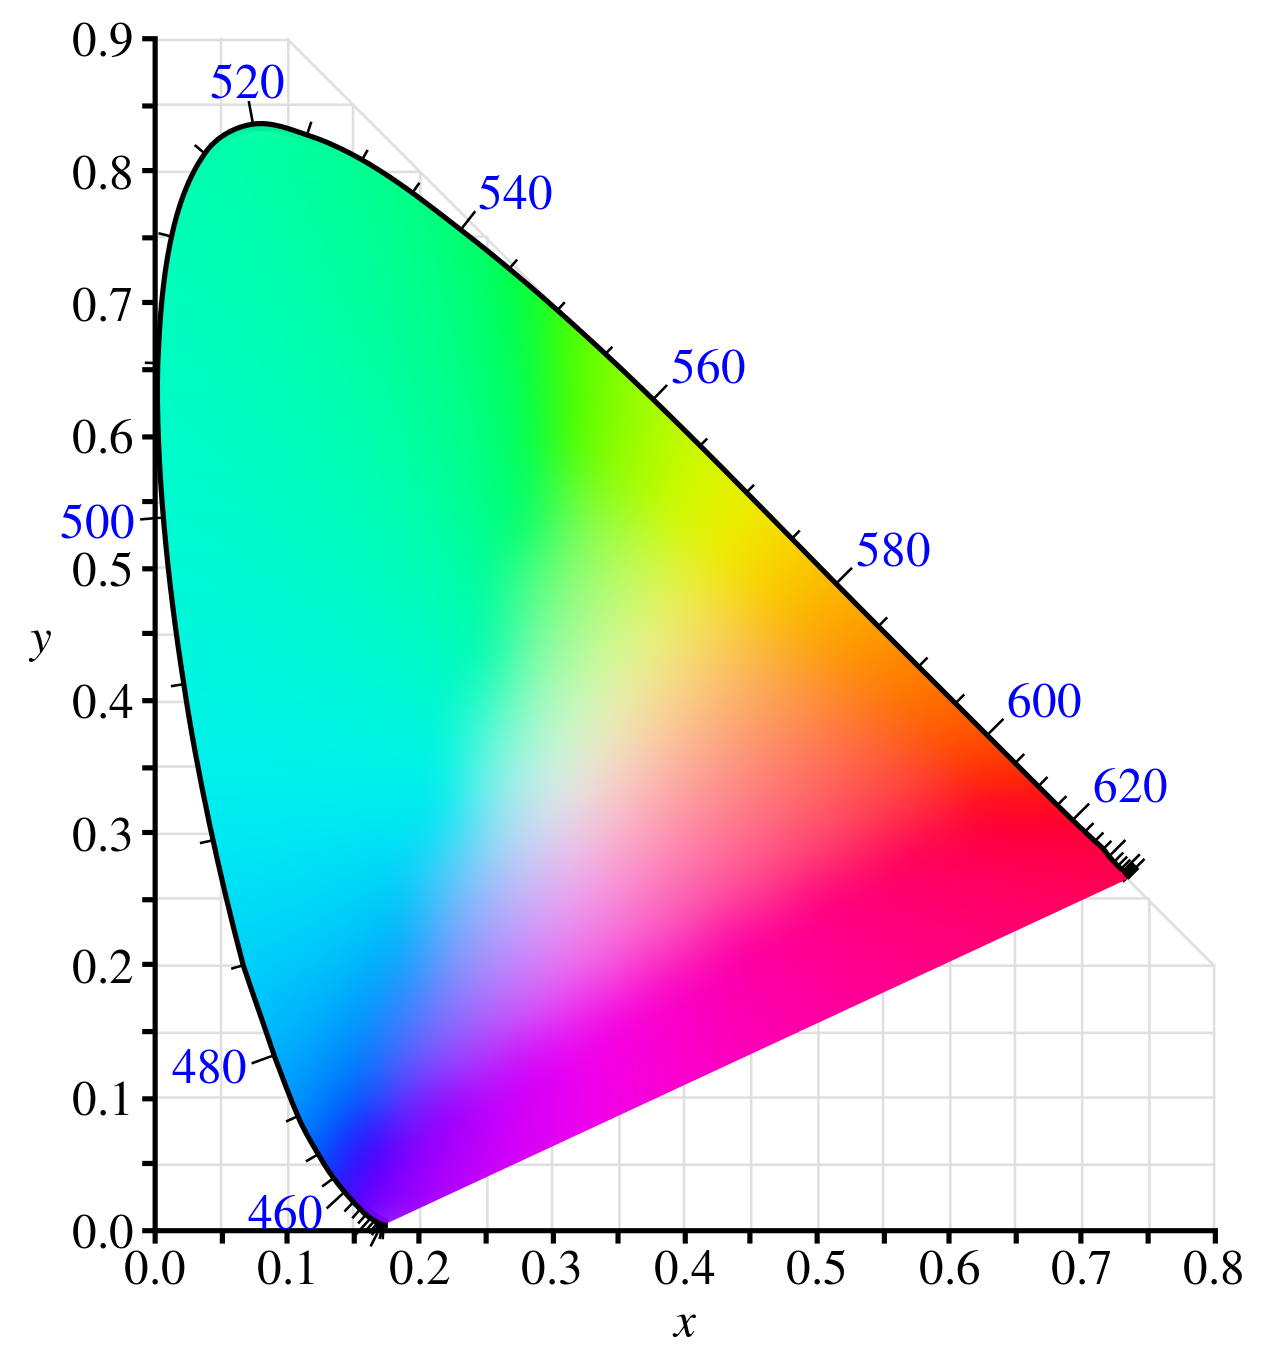
\includegraphics[scale=0.20]{cie.png}
          	\centering
          	\caption{The CIE 1931 color space. Red is at $(0.628,0.346,0.026)$,
            Green is at $(0.268, 0.588,0.144)$, Blue is at $(0.150,0.07,0.780)$}\label{fig:cie}
        \end{figure}
        
    \item the shape must be convex, since any blend (interpolation) of pure
        colors should create a color in the visible region.
    \item the \underline{\textbf{pure colors}} are around the edge of the
        diagram, also called \underline{\textbf{fully saturated}}
    \item the line joining purple and red has no pure equivalent; the colours
        can only be created by blending
    \item \underline{\textbf{Saturation}} of an arbitrary point is the ratio of
        its distance to the white point over the distance of the white point to
        the edge.
    \item white point: when $x=y=z=0.\dot{3}$
    \item The \underline{\textbf{complement color}} of a color is the point
        diametrically opposite through the white point. Computationally, if the
        color has value $(r,g,b)$, its complement color is
        $(255-r,255-g,255-b)$.
    \item The \underline{\textbf{additive primaries}} are RGB (Red, Green, Blue)
        and the \underline{\textbf{subtractive primaries}} are CMY (Cyan,
        Magenta, Yellow).
        Red is the complement color of Cyan, and similarly for Green and Blue,
        as shown in Figure \ref{fig:primaries}.
        \begin{figure}
          	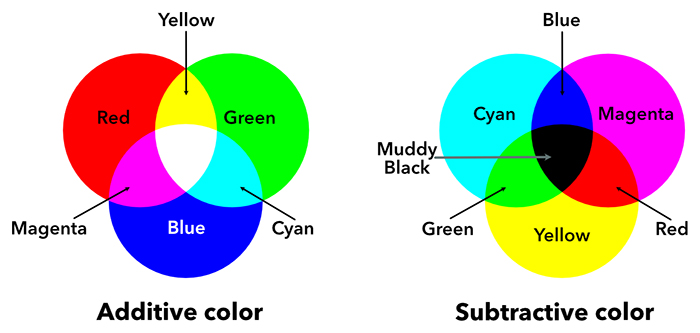
\includegraphics[scale=0.55]{primaries.png}
          	\centering
          	\caption{additive and subtractive primaries}\label{fig:primaries}
        \end{figure}
    \item RGB can be converted to CIE by
        \[
            \begin{pmatrix}
                x \\
                y \\
                z
            \end{pmatrix} 
            =
            \begin{pmatrix}
                0.628 & 0.268 & 0.15 \\
                0.346 & 0.588 & 0.07 \\
                0.026 & 0.144 & 0.78
            \end{pmatrix} 
            \begin{pmatrix}
                r \\
                g \\
                b
            \end{pmatrix} 
        \]
\end{itemize} 

\subsection{HSV Color Representation}

\begin{itemize}
    \item \underline{\textbf{Hue}} corresponds notionally to pure color
    \item \underline{\textbf{Saturation}} is the proportion of pure color
    \item \underline{\textbf{Value}} is the brightness/intensity
\end{itemize} 

\end{document}
